\documentclass[10pt,a4paper]{report}

\usepackage[a4paper,margin=0.72in]{geometry}
\usepackage{graphicx}\usepackage{float}
\usepackage{xcolor}
\usepackage{booktabs}
\usepackage{longtable}
\usepackage{array}
\usepackage{enumitem}
\usepackage{caption}\usepackage{titlesec}
\usepackage{chngcntr}
\usepackage{pdflscape}
\usepackage{listings}
\usepackage{tikz}
\usetikzlibrary{shapes.multipart,calc}
\usepackage[nottoc]{tocbibind}
\usepackage[hidelinks]{hyperref}
\usepackage[strings]{underscore}

\captionsetup{font=small,labelfont=bf}\titlespacing*{\chapter}{0pt}{-8pt}{10pt}\titlespacing*{\section}{0pt}{8pt}{3pt}\titlespacing*{\subsection}{0pt}{6pt}{2pt}
\setlist{itemsep=1pt,topsep=2pt,parsep=0pt}
\renewcommand{\arraystretch}{1.03}
\setlength{\emergencystretch}{3em}

% ---------- code listings ----------
\AtBeginDocument{\counterwithin{lstlisting}{chapter}}
\lstset{
  language=SQL,
  basicstyle=\ttfamily\footnotesize,
  keywordstyle=\bfseries\color{blue!55!black},
  commentstyle=\itshape\color{green!40!black},
  stringstyle=\color{red!50!black},
  frame=single,
  rulecolor=\color{black!40},
  backgroundcolor=\color{black!3},
  breaklines=true,
  breakatwhitespace=false,
  columns=fullflexible,
  keepspaces=true,
  showstringspaces=false,
  numbers=left,
  numberstyle=\tiny\color{black!55},
  numbersep=6pt,
  xleftmargin=1.6em,
  framexleftmargin=1.2em,
  aboveskip=10pt,
  belowskip=6pt,
  captionpos=b,
  morekeywords={ENUM,AUTO_INCREMENT,DATETIME,BIGINT,VARCHAR,DECIMAL,BOOLEAN,CONSTRAINT,CHECK,RESTRICT,CASCADE,UNIQUE,REFERENCES,FOREIGN,START,TRANSACTION,COMMIT,ROLLBACK,LAST_INSERT_ID,SHOW,INDEX,EXPLAIN}
}

% ---------- helper macros ----------
\newcommand{\col}[1]{\texttt{#1}}

% Screenshot helper: drop screenshots/<name>.png next to main.tex and recompile.
\newcommand{\screenshot}[3]{%
  \begin{figure}[htbp]
    \centering
    \IfFileExists{screenshots/#1.png}{%
      \includegraphics[width=#2\textwidth]{screenshots/#1.png}}{%
      \fbox{\parbox[c][6.5cm][c]{0.82\textwidth}{\centering\textit{Screenshot to be inserted}\\[4pt]\texttt{screenshots/#1.png}}}}
    \caption{#3}\label{fig:#1}
  \end{figure}}

\begin{document}

% =====================  TITLE PAGE  =====================
\begin{titlepage}
  \centering
  \thispagestyle{empty}
  \vspace*{1.6cm}
  {\Large\bfseries DATABASE MANAGEMENT SYSTEMS (DBMS)\par}\vspace{1.0cm}

  {\Huge\bfseries Vehicle Rental Management System: A Relational Database Design with MySQL\par}
  \vspace{1.6cm}
  {\Large\bfseries Project Report\par}
  \vspace{1.9cm}

  {\large Submitted by:\par}
  \vspace{0.3cm}
  {\large\bfseries Ritvik Jindal\par}
  Reg No: 2502051953\\
  Programme: B.Tech CSE \hspace{1em} Section: N3
  \vspace{1.6cm}

  {\Large Submitted to:\par}
  \vspace{0.35cm}
  {\LARGE\bfseries Dr. Stuti Pandey\par}

  \vfill
  {\bfseries Department of Computer Science and Engineering\\
  Manipal University Jaipur\par}
  Dehmi Kalan, Near GVK Toll Plaza, Jaipur-Ajmer Expressway,\\
  Jaipur, Rajasthan 303007
\end{titlepage}

% =====================  ABSTRACT  =====================
\pagenumbering{arabic}
\chapter*{Abstract}
\addcontentsline{toc}{chapter}{Abstract}

The Vehicle Rental Management System is a web application for managing vehicle rentals, and this report documents the relational database on which it depends. The objective of the project was to design a normalised MySQL database that stores customers and administrators, vehicles and their images, promotional codes, rental bookings, payments and maintenance records while preserving data integrity. The methodology involved entity-relationship modelling, mapping the model to seven relational tables, and defining primary keys, foreign keys, unique constraints, enumerated types, default values, check constraints and twelve secondary indexes in a MySQL schema script. The design places each entity in its own table, retains the price breakdown of every rental as a historical record, and uses restrictive referential actions to protect rental and payment history. SQL queries for retrieval, aggregation and reporting, together with a transaction pattern for booking and payment, show how the schema supports the main operations of a rental business. The report concludes that a carefully constrained relational schema is a dependable foundation for a rental platform, and it identifies business rules, notably the prevention of overlapping bookings, that should be strengthened in future work.

\bigskip
\noindent\textbf{Keywords:} RDBMS, MySQL, ER diagram, relational schema, normalisation, integrity constraints, indexing, transactions.

\tableofcontents

% =====================  CHAPTERS  =====================
\chapter{Introduction}

\section{Project Overview}
Vehicle rental businesses manage several kinds of connected information: customers who book vehicles, the vehicles themselves together with their images and maintenance histories, promotional offers, rental periods with their price calculations, and online payments. When these facts are kept in separate files or in a single wide table, values are duplicated, updates become inconsistent and orphan records appear. The Vehicle Rental Management System addresses this problem by placing all of this data in a relational database. The system is a web application with a React frontend and a Java-based backend, and this report concentrates on the MySQL database that stores and protects its data.

The database consists of seven tables: \col{users}, \col{vehicles}, \col{vehicle_images}, \col{promo_codes}, \col{rentals}, \col{payments} and \col{maintenance}. Primary and foreign keys connect the tables, and constraints enforce the validity rules the business requires, such as unique registration numbers, non-negative amounts and return times that fall after pickup times.

\section{Objectives of the Project}
The primary objectives of this project were as follows:
\begin{itemize}
  \item To model the entities and relationships involved in vehicle rental operations using an entity-relationship diagram.
  \item To map the model to a relational schema in MySQL with appropriate data types, primary keys and foreign keys.
  \item To enforce data integrity through unique, default, enumerated and check constraints.
  \item To reduce avoidable redundancy by separating related entities into their own tables, and to document any deliberate exceptions.
  \item To provide SQL statements for common retrieval, aggregation and reporting tasks.
  \item To define indexes on the attributes most often used for filtering and joining.
  \item To describe transaction handling for operations that span several tables, such as a booking together with its payment.
\end{itemize}

\section{Importance and Relevance}
A rental platform handles money, schedules and physical assets at the same time. A payment must always belong to a real rental, a rental must always belong to a real customer and vehicle, and the price agreed at booking time must remain available even after the vehicle's current rate changes. These guarantees are best provided by the database itself rather than left entirely to application code. The project therefore demonstrates how keys, constraints, normalisation, indexes and transactions work together in a realistic business domain, and the resulting design can serve as a template for other booking-oriented systems.

\section{Scope and Limitations}
The scope of this report is the relational database layer. It covers the entities and relationships, the relational schema and data dictionary, integrity constraints, normalisation, indexes, representative SQL statements and the use of transactions. The design of the user interface and of the Java service classes is outside the scope of the report.

Limitations of the current database design include:
\begin{itemize}
  \item The schema does not itself prevent two bookings of the same vehicle from overlapping in time; this rule must be enforced by application logic or by additional database code (Section~\ref{sec:transactions}).
  \item \col{payments.user_id} and \col{rentals.user_id} are stored independently, so the schema does not guarantee that a payment's user is the user who owns the rental.
  \item The rules that \col{used_count} must not exceed \col{usage_limit} and that \col{maximum_discount} must be non-negative are not expressed as constraints.
  \item Payment records store Razorpay identifiers only; communication with the payment gateway is handled outside the database and is not covered here.
  \item Refunds are represented only by the \col{REFUNDED} payment status; partial refunds and refund amounts are not modelled.
\end{itemize}

\chapter{System Design}

\section{Database Design Overview}
The heart of the Vehicle Rental Management System is its MySQL database. The design follows the relational model: each table represents one entity, a primary key identifies every row, and foreign keys connect rows across tables so that, for example, a rental cannot exist without a valid user and a valid vehicle. Descriptive data is stored with the entity it describes. Vehicle images, for instance, are kept in their own table so that a vehicle can have any number of images without repeating its other attributes. The schema is created in MySQL 8 and relies on the InnoDB storage engine, which supports foreign keys and transactions \cite{mysqlfk}.

The \col{users} table holds both customers and administrators, distinguished by a role column. The \col{rentals} table is the central table of the design: it links a user to a vehicle for a period of time, records the price calculation, optionally refers to a promotional code, and is the parent of the \col{payments} table.

\section{Entity-Relationship (ER) Diagram}
The ER diagram in Figure~\ref{fig:er} provides a visual blueprint of the database. Each box is an entity with its attributes; primary keys are underlined, foreign keys are in italics, and the labels \textbf{1} and \textbf{N} give the cardinality at each end of a relationship.

The key entities and relationships include:
\begin{itemize}
  \item \textbf{Entities:} User, Vehicle, VehicleImage, PromoCode, Rental, Payment and Maintenance.
  \item \textbf{One-to-Many Relationships:} A \col{User} can make many \col{Rentals} and many \col{Payments}. A \col{Vehicle} can appear in many \col{Rentals} over time and can have many \col{VehicleImages} and many \col{Maintenance} records. A \col{Rental} can have many \col{Payments}. A \col{PromoCode} can be used in many \col{Rentals}.
  \item \textbf{Many-to-Many Relationship:} Users and vehicles are related many-to-many, because a user can rent many vehicles and a vehicle can be rented by many users. The \col{Rental} entity resolves this relationship and also carries the booking attributes (period, price breakdown and status).
  \item \textbf{Optional Relationship:} \col{rentals.promo_id} allows \col{NULL}, since a rental may have no promotional code.
\end{itemize}

\begin{landscape}
\begin{figure}[p]
  \centering
  \resizebox{\linewidth}{!}{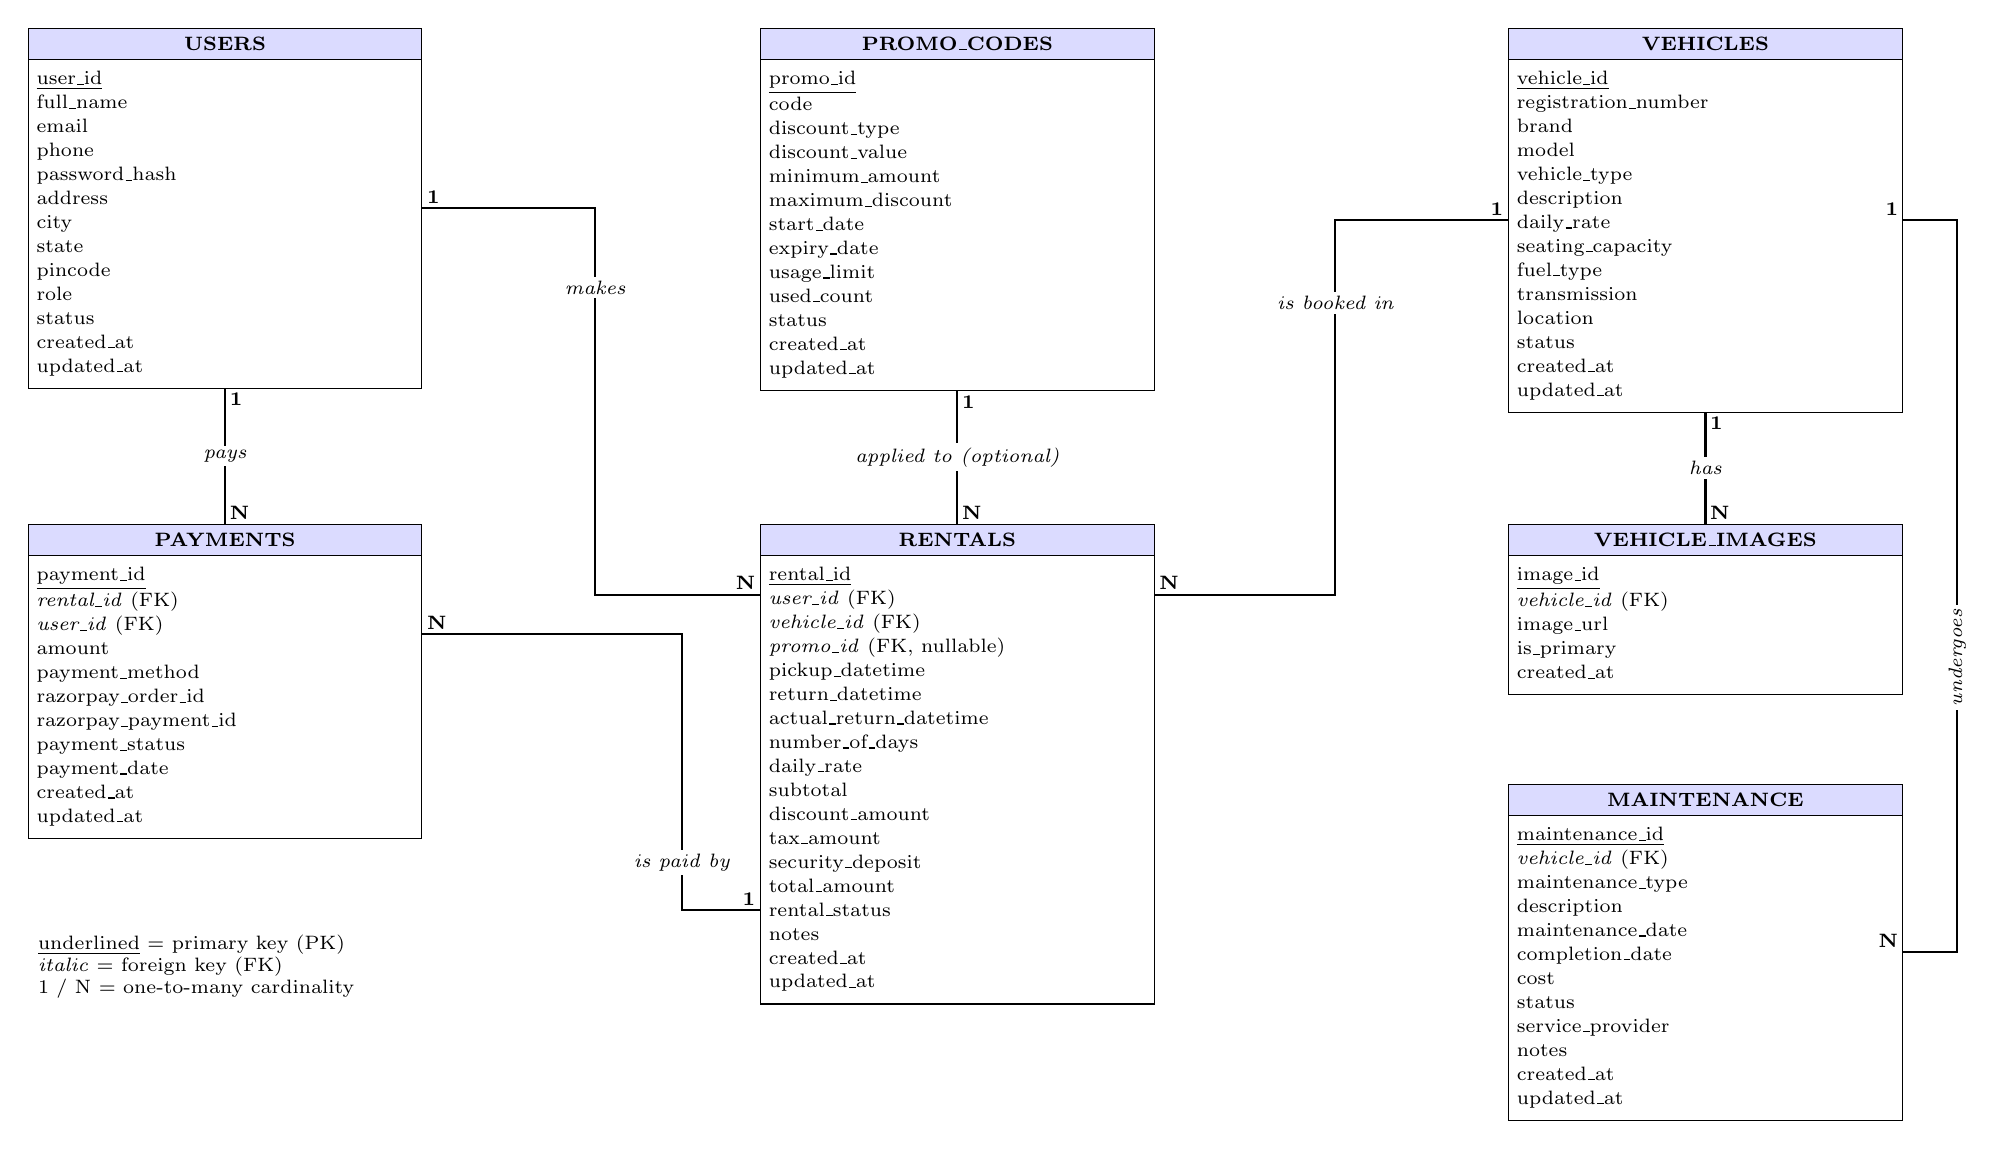
\begin{tikzpicture}[
  ent/.style={draw, rectangle split, rectangle split parts=2,
    rectangle split part fill={blue!14,white}, rectangle split part align={center,left},
    minimum width=5cm, inner sep=3pt, align=left,
    font=\fontsize{7}{8.4}\selectfont},
  card/.style={font=\scriptsize\bfseries, inner sep=1.5pt},
  rel/.style={font=\scriptsize\itshape, fill=white, inner sep=1.5pt},
  link/.style={thick}
]

% ---------- entities ----------
\node[ent, anchor=north] (users) at (2.7,0) {\textbf{USERS}
\nodepart{second}\begin{tabular}{@{}l@{}}
\underline{user\_id}\\ full\_name\\ email\\ phone\\ password\_hash\\ address\\ city\\ state\\ pincode\\ role\\ status\\ created\_at\\ updated\_at
\end{tabular}};

\node[ent, anchor=north] (payments) at (2.7,-6.3) {\textbf{PAYMENTS}
\nodepart{second}\begin{tabular}{@{}l@{}}
\underline{payment\_id}\\ \textit{rental\_id} (FK)\\ \textit{user\_id} (FK)\\ amount\\ payment\_method\\ razorpay\_order\_id\\ razorpay\_payment\_id\\ payment\_status\\ payment\_date\\ created\_at\\ updated\_at
\end{tabular}};

\node[ent, anchor=north] (promo) at (12,0) {\textbf{PROMO\_CODES}
\nodepart{second}\begin{tabular}{@{}l@{}}
\underline{promo\_id}\\ code\\ discount\_type\\ discount\_value\\ minimum\_amount\\ maximum\_discount\\ start\_date\\ expiry\_date\\ usage\_limit\\ used\_count\\ status\\ created\_at\\ updated\_at
\end{tabular}};

\node[ent, anchor=north] (rentals) at (12,-6.3) {\textbf{RENTALS}
\nodepart{second}\begin{tabular}{@{}l@{}}
\underline{rental\_id}\\ \textit{user\_id} (FK)\\ \textit{vehicle\_id} (FK)\\ \textit{promo\_id} (FK, nullable)\\ pickup\_datetime\\ return\_datetime\\ actual\_return\_datetime\\ number\_of\_days\\ daily\_rate\\ subtotal\\ discount\_amount\\ tax\_amount\\ security\_deposit\\ total\_amount\\ rental\_status\\ notes\\ created\_at\\ updated\_at
\end{tabular}};

\node[ent, anchor=north] (vehicles) at (21.5,0) {\textbf{VEHICLES}
\nodepart{second}\begin{tabular}{@{}l@{}}
\underline{vehicle\_id}\\ registration\_number\\ brand\\ model\\ vehicle\_type\\ description\\ daily\_rate\\ seating\_capacity\\ fuel\_type\\ transmission\\ location\\ status\\ created\_at\\ updated\_at
\end{tabular}};

\node[ent, anchor=north] (images) at (21.5,-6.3) {\textbf{VEHICLE\_IMAGES}
\nodepart{second}\begin{tabular}{@{}l@{}}
\underline{image\_id}\\ \textit{vehicle\_id} (FK)\\ image\_url\\ is\_primary\\ created\_at
\end{tabular}};

\node[ent, anchor=north] (maint) at (21.5,-9.6) {\textbf{MAINTENANCE}
\nodepart{second}\begin{tabular}{@{}l@{}}
\underline{maintenance\_id}\\ \textit{vehicle\_id} (FK)\\ maintenance\_type\\ description\\ maintenance\_date\\ completion\_date\\ cost\\ status\\ service\_provider\\ notes\\ created\_at\\ updated\_at
\end{tabular}};

% ---------- relationships ----------
% attachment points on the RENTALS and PAYMENTS boxes
\coordinate (rUser)  at ([yshift=-0.9cm]rentals.north west);
\coordinate (rVeh)   at ([yshift=-0.9cm]rentals.north east);
\coordinate (rPay)   at ([yshift=1.2cm]rentals.south west);
\coordinate (pRent)  at ([yshift=-1.4cm]payments.north east);

% users 1 -- N rentals
\coordinate (xa) at (7.4,0);
\draw[link] (users.east) -- (xa |- users.east) -- (xa |- rUser) -- (rUser);
\node[card, above right] at (users.east) {1};
\node[card, above left] at (rUser) {N};
\node[rel] at (xa |- 0,-3.3) {makes};

% users 1 -- N payments
\draw[link] (users.south) -- (payments.north);
\node[card, below right] at (users.south) {1};
\node[card, above right] at (payments.north) {N};
\node[rel] at ($(users.south)!.5!(payments.north)$) {pays};

% rentals 1 -- N payments
\coordinate (xb) at (8.5,0);
\draw[link] (rPay) -- (xb |- rPay) -- (xb |- pRent) -- (pRent);
\node[card, above left] at (rPay) {1};
\node[card, above right] at (pRent) {N};
\node[rel] at (xb |- 0,-10.6) {is paid by};

% promo_codes 1 -- N rentals (optional)
\draw[link] (promo.south) -- (rentals.north);
\node[card, below right] at (promo.south) {1};
\node[card, above right] at (rentals.north) {N};
\node[rel] at ($(promo.south)!.5!(rentals.north)$) {applied to (optional)};

% vehicles 1 -- N rentals
\coordinate (xc) at (16.8,0);
\draw[link] (vehicles.west) -- (xc |- vehicles.west) -- (xc |- rVeh) -- (rVeh);
\node[card, above left] at (vehicles.west) {1};
\node[card, above right] at (rVeh) {N};
\node[rel] at (xc |- 0,-3.5) {is booked in};

% vehicles 1 -- N vehicle_images
\draw[link] (vehicles.south) -- (images.north);
\node[card, below right] at (vehicles.south) {1};
\node[card, above right] at (images.north) {N};
\node[rel] at ($(vehicles.south)!.5!(images.north)$) {has};

% vehicles 1 -- N maintenance (routed along the right side)
\coordinate (xd) at (24.7,0);
\draw[link] (vehicles.east) -- (xd |- vehicles.east) -- (xd |- maint.east) -- (maint.east);
\node[card, above left] at (vehicles.east) {1};
\node[card, above left] at (maint.east) {N};
\node[rel, rotate=90] at (xd |- 0,-8) {undergoes};

% legend
\node[align=left, font=\scriptsize, anchor=north west] at (0.2,-11.4) {%
\underline{underlined} = primary key (PK)\\ \textit{italic} = foreign key (FK)\\ 1 / N = one-to-many cardinality};
\end{tikzpicture}
}
  \caption{ER Diagram for the Vehicle Rental Management System}
  \label{fig:er}
\end{figure}
\end{landscape}

\section{Relational Schema}
The ER model is mapped to the following relational schema. Primary keys are underlined and foreign keys are shown in italics.
\begin{itemize}
  \item USERS(\underline{user\_id}, full\_name, email, phone, password\_hash, address, city, state, pincode, role, status, created\_at, updated\_at)
  \item VEHICLES(\underline{vehicle\_id}, registration\_number, brand, model, vehicle\_type, description, daily\_rate, seating\_capacity, fuel\_type, transmission, location, status, created\_at, updated\_at)
  \item VEHICLE\_IMAGES(\underline{image\_id}, \textit{vehicle\_id}, image\_url, is\_primary, created\_at)
  \item PROMO\_CODES(\underline{promo\_id}, code, discount\_type, discount\_value, minimum\_amount, maximum\_discount, start\_date, expiry\_date, usage\_limit, used\_count, status, created\_at, updated\_at)
  \item RENTALS(\underline{rental\_id}, \textit{user\_id}, \textit{vehicle\_id}, \textit{promo\_id}, pickup\_datetime, return\_datetime, actual\_return\_datetime, number\_of\_days, daily\_rate, subtotal, discount\_amount, tax\_amount, security\_deposit, total\_amount, rental\_status, notes, created\_at, updated\_at)
  \item PAYMENTS(\underline{payment\_id}, \textit{rental\_id}, \textit{user\_id}, amount, payment\_method, razorpay\_order\_id, razorpay\_payment\_id, payment\_status, payment\_date, created\_at, updated\_at)
  \item MAINTENANCE(\underline{maintenance\_id}, \textit{vehicle\_id}, maintenance\_type, description, maintenance\_date, completion\_date, cost, status, service\_provider, notes, created\_at, updated\_at)
\end{itemize}

Table~\ref{tab:fk} lists the seven foreign-key relationships together with their cardinality and referential actions.

\begin{table}[htbp]
\centering
\small
\caption{Foreign-Key Relationships and Referential Actions}
\label{tab:fk}
\begin{tabular}{@{}lllll@{}}
\toprule
\textbf{Parent} & \textbf{Child.Column} & \textbf{Cardinality} & \textbf{ON DELETE} & \textbf{ON UPDATE} \\
\midrule
users        & rentals.user\_id          & 1:N            & RESTRICT & CASCADE \\
vehicles     & rentals.vehicle\_id       & 1:N            & RESTRICT & CASCADE \\
promo\_codes & rentals.promo\_id         & 1:N (optional) & SET NULL & CASCADE \\
rentals      & payments.rental\_id       & 1:N            & RESTRICT & CASCADE \\
users        & payments.user\_id         & 1:N            & RESTRICT & CASCADE \\
vehicles     & vehicle\_images.vehicle\_id & 1:N          & RESTRICT & CASCADE \\
vehicles     & maintenance.vehicle\_id   & 1:N            & RESTRICT & CASCADE \\
\bottomrule
\end{tabular}
\end{table}

\section{Description of Tables and Attributes}
The schema is composed of the following seven tables, defined in the project's \col{schema.sql} script. In the Key column, PK denotes a primary key, UNI a unique column and FK a foreign key. Unless stated otherwise, a column is \col{NOT NULL}. \col{created_at} and \col{updated_at} are timestamps: the first defaults to the time of insertion and the second is refreshed automatically whenever the row changes.

{\small
\begin{longtable}{@{}llc>{\raggedright\arraybackslash}p{6.6cm}@{}}
\caption{Users Table Schema}\label{tab:users}\\
\toprule \textbf{Field} & \textbf{Type} & \textbf{Key} & \textbf{Description}\\ \midrule \endfirsthead
\toprule \textbf{Field} & \textbf{Type} & \textbf{Key} & \textbf{Description}\\ \midrule \endhead
\bottomrule \endfoot
\col{user_id} & BIGINT & PK & Unique identifier; auto-increment.\\
\col{full_name} & VARCHAR(100) & & User's full name.\\
\col{email} & VARCHAR(150) & UNI & Email address.\\
\col{phone} & VARCHAR(20) & UNI & Phone number.\\
\col{password_hash} & VARCHAR(255) & & Hashed password; no plain-text password is stored.\\
\col{address} & VARCHAR(255) & & Street address; optional.\\
\col{city} & VARCHAR(100) & & City; optional.\\
\col{state} & VARCHAR(100) & & State; optional.\\
\col{pincode} & VARCHAR(10) & & Postal code stored as text; optional.\\
\col{role} & ENUM & & \col{CUSTOMER} or \col{ADMIN}; default \col{CUSTOMER}.\\
\col{status} & ENUM & & \col{ACTIVE} or \col{INACTIVE}; default \col{ACTIVE}.\\
\col{created_at} & DATETIME & & Creation timestamp.\\
\col{updated_at} & DATETIME & & Last-update timestamp.\\
\end{longtable}

\begin{longtable}{@{}llc>{\raggedright\arraybackslash}p{6.6cm}@{}}
\caption{Vehicles Table Schema}\label{tab:vehicles}\\
\toprule \textbf{Field} & \textbf{Type} & \textbf{Key} & \textbf{Description}\\ \midrule \endfirsthead
\toprule \textbf{Field} & \textbf{Type} & \textbf{Key} & \textbf{Description}\\ \midrule \endhead
\bottomrule \endfoot
\col{vehicle_id} & BIGINT & PK & Unique identifier; auto-increment.\\
\col{registration_number} & VARCHAR(30) & UNI & Vehicle registration number.\\
\col{brand} & VARCHAR(80) & & Manufacturer or brand.\\
\col{model} & VARCHAR(100) & & Vehicle model.\\
\col{vehicle_type} & ENUM & & \col{CAR}, \col{BIKE}, \col{BUS} or \col{TRUCK}.\\
\col{description} & TEXT & & Free-text description; optional.\\
\col{daily_rate} & DECIMAL(10,2) & & Current rental rate per day; must be $\geq 0$.\\
\col{seating_capacity} & INT & & Number of seats; must be $> 0$.\\
\col{fuel_type} & ENUM & & \col{PETROL}, \col{DIESEL}, \col{ELECTRIC}, \col{CNG} or \col{HYBRID}.\\
\col{transmission} & ENUM & & \col{MANUAL}, \col{AUTOMATIC} or \col{NOT_APPLICABLE}; nullable, default \col{NOT_APPLICABLE}.\\
\col{location} & VARCHAR(150) & & Location where the vehicle is available.\\
\col{status} & ENUM & & \col{AVAILABLE}, \col{RENTED}, \col{MAINTENANCE} or \col{INACTIVE}; default \col{AVAILABLE}.\\
\col{created_at} & DATETIME & & Creation timestamp.\\
\col{updated_at} & DATETIME & & Last-update timestamp.\\
\end{longtable}

\begin{longtable}{@{}llc>{\raggedright\arraybackslash}p{6.6cm}@{}}
\caption{Vehicle Images Table Schema}\label{tab:images}\\
\toprule \textbf{Field} & \textbf{Type} & \textbf{Key} & \textbf{Description}\\ \midrule \endfirsthead
\toprule \textbf{Field} & \textbf{Type} & \textbf{Key} & \textbf{Description}\\ \midrule \endhead
\bottomrule \endfoot
\col{image_id} & BIGINT & PK & Unique identifier; auto-increment.\\
\col{vehicle_id} & BIGINT & FK & References \col{vehicles(vehicle_id)}.\\
\col{image_url} & VARCHAR(500) & & Location (URL) of the image.\\
\col{is_primary} & BOOLEAN & & Marks the primary image; default \col{FALSE}.\\
\col{created_at} & DATETIME & & Creation timestamp.\\
\end{longtable}

\begin{longtable}{@{}llc>{\raggedright\arraybackslash}p{6.6cm}@{}}
\caption{Promo Codes Table Schema}\label{tab:promo}\\
\toprule \textbf{Field} & \textbf{Type} & \textbf{Key} & \textbf{Description}\\ \midrule \endfirsthead
\toprule \textbf{Field} & \textbf{Type} & \textbf{Key} & \textbf{Description}\\ \midrule \endhead
\bottomrule \endfoot
\col{promo_id} & BIGINT & PK & Unique identifier; auto-increment.\\
\col{code} & VARCHAR(50) & UNI & Promotional code entered by the customer.\\
\col{discount_type} & ENUM & & \col{PERCENTAGE} or \col{FIXED}.\\
\col{discount_value} & DECIMAL(10,2) & & Discount amount or percentage; must be $\geq 0$.\\
\col{minimum_amount} & DECIMAL(10,2) & & Minimum booking amount for the code; default 0, must be $\geq 0$.\\
\col{maximum_discount} & DECIMAL(10,2) & & Upper limit on the discount; optional.\\
\col{start_date} & DATE & & First valid date.\\
\col{expiry_date} & DATE & & Last valid date; must not precede \col{start_date}.\\
\col{usage_limit} & INT & & Maximum number of uses; optional, must be $> 0$ if present.\\
\col{used_count} & INT & & Number of times used; default 0.\\
\col{status} & ENUM & & \col{ACTIVE} or \col{INACTIVE}; default \col{ACTIVE}.\\
\col{created_at} & DATETIME & & Creation timestamp.\\
\col{updated_at} & DATETIME & & Last-update timestamp.\\
\end{longtable}

\begin{longtable}{@{}llc>{\raggedright\arraybackslash}p{6.6cm}@{}}
\caption{Rentals Table Schema}\label{tab:rentals}\\
\toprule \textbf{Field} & \textbf{Type} & \textbf{Key} & \textbf{Description}\\ \midrule \endfirsthead
\toprule \textbf{Field} & \textbf{Type} & \textbf{Key} & \textbf{Description}\\ \midrule \endhead
\bottomrule \endfoot
\col{rental_id} & BIGINT & PK & Unique identifier; auto-increment.\\
\col{user_id} & BIGINT & FK & References \col{users(user_id)}.\\
\col{vehicle_id} & BIGINT & FK & References \col{vehicles(vehicle_id)}.\\
\col{promo_id} & BIGINT & FK & References \col{promo_codes(promo_id)}; nullable.\\
\col{pickup_datetime} & DATETIME & & Planned pickup date and time.\\
\col{return_datetime} & DATETIME & & Planned return; must be later than pickup.\\
\col{actual_return_datetime} & DATETIME & & Actual return time; nullable until the vehicle is returned.\\
\col{number_of_days} & INT & & Number of rental days; must be $> 0$.\\
\col{daily_rate} & DECIMAL(10,2) & & Daily rate agreed at booking time; must be $\geq 0$.\\
\col{subtotal} & DECIMAL(10,2) & & Price before discount and tax; must be $\geq 0$.\\
\col{discount_amount} & DECIMAL(10,2) & & Discount applied; default 0, must be $\geq 0$.\\
\col{tax_amount} & DECIMAL(10,2) & & Tax charged; default 0, must be $\geq 0$.\\
\col{security_deposit} & DECIMAL(10,2) & & Deposit collected; default 0, must be $\geq 0$.\\
\col{total_amount} & DECIMAL(10,2) & & Total payable; must be $\geq 0$.\\
\col{rental_status} & ENUM & & \col{PENDING}, \col{CONFIRMED}, \col{ACTIVE}, \col{COMPLETED} or \col{CANCELLED}; default \col{PENDING}.\\
\col{notes} & TEXT & & Booking notes; optional.\\
\col{created_at} & DATETIME & & Creation timestamp.\\
\col{updated_at} & DATETIME & & Last-update timestamp.\\
\end{longtable}

\begin{longtable}{@{}llc>{\raggedright\arraybackslash}p{6.6cm}@{}}
\caption{Payments Table Schema}\label{tab:payments}\\
\toprule \textbf{Field} & \textbf{Type} & \textbf{Key} & \textbf{Description}\\ \midrule \endfirsthead
\toprule \textbf{Field} & \textbf{Type} & \textbf{Key} & \textbf{Description}\\ \midrule \endhead
\bottomrule \endfoot
\col{payment_id} & BIGINT & PK & Unique identifier; auto-increment.\\
\col{rental_id} & BIGINT & FK & References \col{rentals(rental_id)}.\\
\col{user_id} & BIGINT & FK & References \col{users(user_id)}.\\
\col{amount} & DECIMAL(10,2) & & Payment amount; must be $> 0$.\\
\col{payment_method} & ENUM & & Currently only \col{RAZORPAY}; default \col{RAZORPAY}.\\
\col{razorpay_order_id} & VARCHAR(100) & UNI & Provider order identifier; nullable.\\
\col{razorpay_payment_id} & VARCHAR(100) & UNI & Provider payment identifier; nullable.\\
\col{payment_status} & ENUM & & \col{PENDING}, \col{SUCCESS}, \col{FAILED}, \col{CANCELLED} or \col{REFUNDED}; default \col{PENDING}.\\
\col{payment_date} & DATETIME & & Date and time of payment; nullable.\\
\col{created_at} & DATETIME & & Creation timestamp.\\
\col{updated_at} & DATETIME & & Last-update timestamp.\\
\end{longtable}

\begin{longtable}{@{}llc>{\raggedright\arraybackslash}p{6.6cm}@{}}
\caption{Maintenance Table Schema}\label{tab:maintenance}\\
\toprule \textbf{Field} & \textbf{Type} & \textbf{Key} & \textbf{Description}\\ \midrule \endfirsthead
\toprule \textbf{Field} & \textbf{Type} & \textbf{Key} & \textbf{Description}\\ \midrule \endhead
\bottomrule \endfoot
\col{maintenance_id} & BIGINT & PK & Unique identifier; auto-increment.\\
\col{vehicle_id} & BIGINT & FK & References \col{vehicles(vehicle_id)}.\\
\col{maintenance_type} & VARCHAR(100) & & Type of maintenance work.\\
\col{description} & TEXT & & Description of the work; optional.\\
\col{maintenance_date} & DATE & & Date the maintenance is scheduled or starts.\\
\col{completion_date} & DATE & & Completion date; nullable, not earlier than \col{maintenance_date}.\\
\col{cost} & DECIMAL(10,2) & & Cost of the work; default 0, must be $\geq 0$.\\
\col{status} & ENUM & & \col{SCHEDULED}, \col{IN_PROGRESS}, \col{COMPLETED} or \col{CANCELLED}; default \col{SCHEDULED}.\\
\col{service_provider} & VARCHAR(150) & & Workshop or provider; optional.\\
\col{notes} & TEXT & & Additional notes; optional.\\
\col{created_at} & DATETIME & & Creation timestamp.\\
\col{updated_at} & DATETIME & & Last-update timestamp.\\
\end{longtable}
}

\section{Keys and Integrity Constraints}

\subsection{Primary Keys}
Every table has a primary key consisting of an auto-incrementing \col{BIGINT} identifier: \col{user_id}, \col{vehicle_id}, \col{image_id}, \col{promo_id}, \col{rental_id}, \col{payment_id} and \col{maintenance_id}. Primary keys identify rows uniquely and cannot be \col{NULL}.

\subsection{Unique Constraints}
Unique constraints are defined on \col{users.email}, \col{users.phone}, \col{vehicles.registration_number}, \col{promo_codes.code}, \col{payments.razorpay_order_id} and \col{payments.razorpay_payment_id}. They prevent duplicate accounts, duplicate vehicles, duplicate promotional codes and duplicate payment-provider identifiers. In MySQL a unique index permits multiple \col{NULL} values, so payment records without a provider identifier do not conflict with one another.

\subsection{Foreign Keys}
Seven foreign keys connect the tables (Table~\ref{tab:fk}). Six use \col{ON DELETE RESTRICT}, which prevents a parent row from being deleted while dependent rows exist, so a vehicle with rental history cannot be removed accidentally. The foreign key from \col{rentals.promo_id} uses \col{ON DELETE SET NULL}, so deleting a promotional code leaves the rental in place with a \col{NULL} promo reference. All seven use \col{ON UPDATE CASCADE}, which propagates a change of a parent key to the child rows.

\subsection{Check Constraints}
Check constraints express basic validity rules for amounts, counts and dates. The schema defines seventeen named checks, summarised in Table~\ref{tab:checks}. MySQL enforces \col{CHECK} constraints from version 8.0.16 onwards \cite{mysqlcreate}.

\begin{table}[htbp]
\centering
\small
\caption{Check Constraints in the Schema}
\label{tab:checks}
\begin{tabular}{@{}lll@{}}
\toprule
\textbf{Table} & \textbf{Constraint} & \textbf{Rule} \\
\midrule
vehicles & \col{chk_daily_rate} & daily\_rate $\geq 0$ \\
vehicles & \col{chk_seating_capacity} & seating\_capacity $> 0$ \\
promo\_codes & \col{chk_discount_value} & discount\_value $\geq 0$ \\
promo\_codes & \col{chk_minimum_amount} & minimum\_amount $\geq 0$ \\
promo\_codes & \col{chk_usage_limit} & usage\_limit is \col{NULL} or $> 0$ \\
promo\_codes & \col{chk_expiry_date} & expiry\_date $\geq$ start\_date \\
rentals & \col{chk_return_datetime} & return\_datetime $>$ pickup\_datetime \\
rentals & \col{chk_number_of_days} & number\_of\_days $> 0$ \\
rentals & \col{chk_rental_daily_rate} & daily\_rate $\geq 0$ \\
rentals & \col{chk_subtotal} & subtotal $\geq 0$ \\
rentals & \col{chk_discount_amount} & discount\_amount $\geq 0$ \\
rentals & \col{chk_tax_amount} & tax\_amount $\geq 0$ \\
rentals & \col{chk_security_deposit} & security\_deposit $\geq 0$ \\
rentals & \col{chk_total_amount} & total\_amount $\geq 0$ \\
payments & \col{chk_payment_amount} & amount $> 0$ \\
maintenance & \col{chk_maintenance_cost} & cost $\geq 0$ \\
maintenance & \col{chk_completion_date} & completion\_date is \col{NULL} or $\geq$ maintenance\_date \\
\bottomrule
\end{tabular}
\end{table}

\subsection{Domain Constraints}
Enumerated columns (\col{role}, \col{vehicle_type}, \col{fuel_type}, \col{rental_status}, \col{payment_status} and others) restrict a column to a fixed set of values, \col{NOT NULL} makes a value mandatory, and default values supply common states such as \col{PENDING} for a new rental or \col{AVAILABLE} for a new vehicle.

\section{Normalisation}
Normalisation structures relations so that each fact is stored once, which reduces redundancy and update anomalies \cite{silberschatz,elmasri}. Table~\ref{tab:fds} lists the candidate keys and the dependency of the remaining attributes for each table.

\begin{table}[htbp]
\centering
\small
\caption{Candidate Keys and Functional Dependencies}
\label{tab:fds}
\begin{tabular}{@{}l>{\raggedright\arraybackslash}p{4.3cm}>{\raggedright\arraybackslash}p{6.2cm}@{}}
\toprule
\textbf{Table} & \textbf{Candidate keys} & \textbf{Functional dependencies} \\
\midrule
users & user\_id, email, phone & Each candidate key determines all other attributes. \\
vehicles & vehicle\_id, registration\_number & Each candidate key determines all other attributes. \\
vehicle\_images & image\_id & image\_id $\rightarrow$ all other attributes. \\
promo\_codes & promo\_id, code & Each candidate key determines all other attributes. \\
rentals & rental\_id & rental\_id $\rightarrow$ all other attributes. \\
payments & payment\_id (also the provider identifiers when present) & payment\_id $\rightarrow$ all other attributes. \\
maintenance & maintenance\_id & maintenance\_id $\rightarrow$ all other attributes. \\
\bottomrule
\end{tabular}
\end{table}

\subsection{First Normal Form (1NF)}
All attributes hold single, atomic values and there are no repeating groups. Instead of storing a list of image links in a vehicle row, each image is a separate row in \col{vehicle_images}. Rentals, payments and maintenance records are likewise stored as separate rows rather than as multi-valued columns.

\subsection{Second Normal Form (2NF)}
Every table has a single-column primary key, so no non-key attribute can depend on only part of a key. All tables that are in 1NF are therefore also in 2NF. Descriptive data is held with its own entity: vehicle characteristics in \col{vehicles}, contact details in \col{users} and work details in \col{maintenance}.

\subsection{Third Normal Form (3NF)}
A relation is in 3NF when no non-key attribute depends on the key through another non-key attribute. Brand and model are stored once in \col{vehicles} and are not copied into each rental; user contact data is stored once in \col{users}; promotion rules are stored once in \col{promo_codes}. Table~\ref{tab:nf} summarises the result for each table, including three deliberate exceptions.

\begin{table}[htbp]
\centering
\small
\caption{Normal Form Achieved by Each Table}
\label{tab:nf}
\begin{tabular}{@{}lc>{\raggedright\arraybackslash}p{8.4cm}@{}}
\toprule
\textbf{Table} & \textbf{Normal form} & \textbf{Notes and exceptions} \\
\midrule
users & 3NF* & *If a postal code is taken to determine city and state, \col{pincode} $\rightarrow$ \col{city}, \col{state} is a transitive dependency. The three columns are kept together because addresses are entered by users and are optional. \\
vehicles & 3NF & \col{status} records the current operational state. The value \col{RENTED} can also be derived from \col{rentals}; it is retained for fast availability lookups. \\
vehicle\_images & 3NF & No exceptions. \\
promo\_codes & 3NF & No exceptions. \\
rentals & 3NF* & *\col{number_of_days}, \col{daily_rate}, \col{subtotal} and \col{total_amount} are stored as a snapshot of the booking. They are not recomputed from the vehicle's current rate, which may change after the booking. \\
payments & 3NF* & *\col{user_id} can normally be derived from the rental. It is stored so that payments can be queried directly by user. \\
maintenance & 3NF & No exceptions. \\
\bottomrule
\end{tabular}
\end{table}

\subsection{Benefits of Normalisation}
\begin{itemize}
  \item A user can change contact details without touching any rental record.
  \item Vehicle information is maintained in one place while rental history remains intact.
  \item Several images, payments and maintenance records can be attached to one vehicle or rental without duplicating descriptive data.
  \item Promotion rules can be changed once without editing every rental that used them.
\end{itemize}

\section{Indexes}
An index is an auxiliary structure that lets MySQL find rows without scanning a whole table. Primary keys and unique constraints are indexed automatically. In addition, the schema script creates twelve secondary indexes (Table~\ref{tab:indexes}) on columns that are frequently used in filters and joins. Each index is created only if an index of the same name does not already exist, by checking \col{information_schema.statistics} before executing the \col{CREATE INDEX} statement, so the script can be run again safely against an existing database. The foreign-key columns \col{rentals.promo_id} and \col{vehicle_images.vehicle_id} have no explicit index; InnoDB creates an index for them automatically because a foreign key requires one \cite{mysqlfk}.

Indexes use storage and add work to every insert and update, so they should be chosen to match real query patterns. The \col{EXPLAIN} statement can be used to confirm that a query uses an intended index \cite{mysqlindex}.

\begin{table}[htbp]
\centering
\small
\caption{Secondary Indexes Defined in the Schema}
\label{tab:indexes}
\begin{tabular}{@{}lll@{}}
\toprule
\textbf{Index} & \textbf{Column} & \textbf{Typical use} \\
\midrule
\col{idx_vehicle_type} & vehicles.vehicle\_type & Filtering by vehicle category \\
\col{idx_vehicle_status} & vehicles.status & Listing vehicles by availability \\
\col{idx_vehicle_location} & vehicles.location & Filtering by location \\
\col{idx_rental_user} & rentals.user\_id & Retrieving a user's rentals \\
\col{idx_rental_vehicle} & rentals.vehicle\_id & Retrieving rentals of a vehicle \\
\col{idx_rental_status} & rentals.rental\_status & Filtering rentals by status \\
\col{idx_rental_pickup} & rentals.pickup\_datetime & Date-range queries on pickup \\
\col{idx_rental_return} & rentals.return\_datetime & Date-range queries on return \\
\col{idx_payment_rental} & payments.rental\_id & Retrieving payments of a rental \\
\col{idx_payment_user} & payments.user\_id & Retrieving payments of a user \\
\col{idx_maintenance_vehicle} & maintenance.vehicle\_id & Maintenance history of a vehicle \\
\col{idx_maintenance_status} & maintenance.status & Filtering maintenance by status \\
\bottomrule
\end{tabular}
\end{table}

\chapter{Database Implementation}

\section{Database Environment}
The database is named \col{vehicle_rental_db} and is defined in MySQL by the \col{schema.sql} script. The script uses the MySQL types \col{BIGINT}, \col{VARCHAR}, \col{DECIMAL}, \col{DATETIME}, \col{DATE}, \col{TEXT}, \col{BOOLEAN} and \col{ENUM}. Every table is created with \col{CREATE TABLE IF NOT EXISTS}, so running the script against a database that already contains the tables does not fail. The script requires MySQL 8.0.16 or later, the first release that enforces \col{CHECK} constraints \cite{mysqlcreate}. The statements in this chapter can be run in MySQL Workbench or any other MySQL client.

\section{SQL Data Definition Language (DDL)}
Data Definition Language statements create and change the structure of the database. Listing~\ref{lst:ddl} shows the definition of the \col{vehicles} table, which illustrates primary keys, unique and \col{NOT NULL} columns, enumerated types, defaults and named check constraints.

\begin{lstlisting}[caption={DDL for the vehicles table},label={lst:ddl}]
CREATE TABLE IF NOT EXISTS vehicles (
    vehicle_id BIGINT AUTO_INCREMENT PRIMARY KEY,
    registration_number VARCHAR(30) NOT NULL UNIQUE,
    brand VARCHAR(80) NOT NULL,
    model VARCHAR(100) NOT NULL,
    vehicle_type ENUM('CAR','BIKE','BUS','TRUCK') NOT NULL,
    description TEXT,
    daily_rate DECIMAL(10,2) NOT NULL,
    seating_capacity INT NOT NULL,
    fuel_type ENUM('PETROL','DIESEL','ELECTRIC','CNG','HYBRID') NOT NULL,
    transmission ENUM('MANUAL','AUTOMATIC','NOT_APPLICABLE')
        DEFAULT 'NOT_APPLICABLE',
    location VARCHAR(150) NOT NULL,
    status ENUM('AVAILABLE','RENTED','MAINTENANCE','INACTIVE')
        NOT NULL DEFAULT 'AVAILABLE',
    created_at DATETIME NOT NULL DEFAULT CURRENT_TIMESTAMP,
    updated_at DATETIME NOT NULL DEFAULT CURRENT_TIMESTAMP
        ON UPDATE CURRENT_TIMESTAMP,
    CONSTRAINT chk_daily_rate CHECK (daily_rate >= 0),
    CONSTRAINT chk_seating_capacity CHECK (seating_capacity > 0)
);
\end{lstlisting}

The secondary indexes are created by statements that first check the metadata, as shown in Listing~\ref{lst:index}.

\begin{lstlisting}[caption={Idempotent creation of an index},label={lst:index}]
SET @sql := IF(NOT EXISTS (
    SELECT 1 FROM information_schema.statistics
    WHERE table_schema = DATABASE()
      AND table_name = 'vehicles'
      AND index_name = 'idx_vehicle_status'),
  'CREATE INDEX idx_vehicle_status ON vehicles(status)',
  'DO 0');
PREPARE stmt FROM @sql;
EXECUTE stmt;
DEALLOCATE PREPARE stmt;
\end{lstlisting}

\section{SQL Data Manipulation Language (DML)}
Data Manipulation Language statements insert, change and remove rows. The statements below use example values; the identifiers must correspond to existing rows when they are executed.

\begin{lstlisting}[caption={Inserting a vehicle},label={lst:insert}]
INSERT INTO vehicles
  (registration_number, brand, model, vehicle_type,
   daily_rate, seating_capacity, fuel_type, transmission,
   location, status)
VALUES
  ('RJ14AB1234', 'Maruti', 'Swift', 'CAR',
   1800.00, 5, 'PETROL', 'MANUAL', 'Jaipur', 'AVAILABLE');
\end{lstlisting}

\begin{lstlisting}[caption={Updating and deleting rows},label={lst:updatedelete}]
-- Mark a vehicle as under maintenance
UPDATE vehicles
SET status = 'MAINTENANCE'
WHERE vehicle_id = 1;

-- Remove an image that is no longer needed
DELETE FROM vehicle_images
WHERE image_id = 1;
\end{lstlisting}

A \col{DELETE} on a parent row such as a vehicle that still has rentals is rejected by the foreign-key rules (Section~\ref{sec:refactions}); an inactive status is used when history must be preserved.

\section{SQL Retrieval Queries}
The following queries show typical retrieval and reporting operations. They only read data and do not change the database.

\subsubsection{List Available Vehicles}
\begin{lstlisting}[caption={Filtering and sorting vehicles},label={lst:q1}]
SELECT vehicle_id, brand, model, vehicle_type,
       daily_rate, location
FROM vehicles
WHERE status = 'AVAILABLE'
ORDER BY daily_rate ASC;
\end{lstlisting}
The query filters vehicles by status and lists them from the lowest to the highest daily rate. It can use \col{idx_vehicle_status}.

\subsubsection{Find Rentals of a User}
\begin{lstlisting}[caption={Joining users and rentals},label={lst:q2}]
SELECT u.full_name, r.rental_id,
       r.pickup_datetime, r.return_datetime,
       r.total_amount, r.rental_status
FROM users AS u
JOIN rentals AS r ON r.user_id = u.user_id
WHERE u.user_id = 1
ORDER BY r.created_at DESC;
\end{lstlisting}
The inner join matches every rental with the user referenced by its foreign key.

\subsubsection{View Payments of a Rental}
\begin{lstlisting}[caption={Joining rentals and payments},label={lst:q3}]
SELECT r.rental_id, p.payment_id, p.amount,
       p.payment_method, p.payment_status, p.payment_date
FROM rentals AS r
JOIN payments AS p ON p.rental_id = r.rental_id
WHERE r.rental_id = 1
ORDER BY p.created_at DESC;
\end{lstlisting}

\subsubsection{Count Rentals by Status}
\begin{lstlisting}[caption={Aggregation with GROUP BY},label={lst:q4}]
SELECT rental_status, COUNT(*) AS rental_count
FROM rentals
GROUP BY rental_status
ORDER BY rental_count DESC;
\end{lstlisting}

\subsubsection{Total of Successful Payments per User}
\begin{lstlisting}[caption={SUM with a status filter},label={lst:q5}]
SELECT user_id, SUM(amount) AS successful_total
FROM payments
WHERE payment_status = 'SUCCESS'
GROUP BY user_id
ORDER BY successful_total DESC;
\end{lstlisting}
The result is a report of the payment rows recorded as successful in the database.

\subsubsection{Maintenance History of a Vehicle}
\begin{lstlisting}[caption={Joining vehicles and maintenance},label={lst:q6}]
SELECT v.registration_number, v.brand, v.model,
       m.maintenance_type, m.maintenance_date,
       m.completion_date, m.cost, m.status
FROM vehicles AS v
JOIN maintenance AS m ON m.vehicle_id = v.vehicle_id
WHERE v.vehicle_id = 1
ORDER BY m.maintenance_date DESC;
\end{lstlisting}

\subsubsection{Rentals with Optional Promo Codes}
\begin{lstlisting}[caption={LEFT JOIN for an optional relationship},label={lst:q7}]
SELECT r.rental_id, r.total_amount,
       pc.code, pc.discount_type, r.discount_amount
FROM rentals AS r
LEFT JOIN promo_codes AS pc ON pc.promo_id = r.promo_id
ORDER BY r.created_at DESC;
\end{lstlisting}
A \col{LEFT JOIN} is used because \col{rentals.promo_id} is nullable: rentals without a promo code stay in the result with \col{NULL} promo columns.

\subsubsection{Vehicles That Have Never Been Rented}
\begin{lstlisting}[caption={Subquery with NOT IN},label={lst:q8}]
SELECT vehicle_id, registration_number, brand, model
FROM vehicles
WHERE vehicle_id NOT IN (SELECT vehicle_id FROM rentals);
\end{lstlisting}

\subsubsection{Customers with Repeat Completed Rentals}
\begin{lstlisting}[caption={GROUP BY with HAVING},label={lst:q9}]
SELECT u.user_id, u.full_name, COUNT(*) AS completed_rentals
FROM users AS u
JOIN rentals AS r ON r.user_id = u.user_id
WHERE r.rental_status = 'COMPLETED'
GROUP BY u.user_id, u.full_name
HAVING COUNT(*) >= 2
ORDER BY completed_rentals DESC;
\end{lstlisting}

\subsection{Query Concepts Used}
The queries demonstrate \col{WHERE} for filtering, \col{ORDER BY} for sorting, \col{INNER JOIN} and \col{LEFT JOIN} for combining related tables, \col{COUNT} and \col{SUM} for aggregation, \col{GROUP BY} and \col{HAVING} for grouped summaries, and a subquery with \col{NOT IN}.

\section{Transactions and ACID Properties}\label{sec:transactions}
A transaction groups several database operations into one logical unit. Creating a rental and recording its payment is a typical example, because either both records must exist or neither should. Transactions provide the ACID properties:
\begin{itemize}
  \item \textbf{Atomicity:} all statements of the transaction take effect, or none of them do.
  \item \textbf{Consistency:} integrity constraints hold before and after the transaction.
  \item \textbf{Isolation:} concurrent transactions do not interfere in ways that break correctness.
  \item \textbf{Durability:} committed changes persist.
\end{itemize}

Listing~\ref{lst:txn} shows a booking transaction. The vehicle row is locked first, so that concurrent bookings of the same vehicle are processed one after another by InnoDB. The overlap check is then executed, and the rental and payment are inserted only if no overlapping booking is found. The monetary values and identifiers are examples, and the totals are calculated by the application.

\begin{lstlisting}[caption={Booking transaction for a rental and its payment},label={lst:txn}]
START TRANSACTION;

-- 1. Lock the vehicle row so concurrent bookings are serialised
SELECT vehicle_id FROM vehicles
WHERE vehicle_id = 1 AND status <> 'INACTIVE'
FOR UPDATE;

-- 2. Check for overlapping bookings (continue only if the count is 0)
SELECT COUNT(*) AS overlapping
FROM rentals
WHERE vehicle_id = 1
  AND rental_status IN ('PENDING','CONFIRMED','ACTIVE')
  AND pickup_datetime < '2026-11-05 10:00:00'
  AND return_datetime > '2026-11-01 10:00:00';

-- 3. Create the rental
INSERT INTO rentals
  (user_id, vehicle_id, pickup_datetime, return_datetime,
   number_of_days, daily_rate, subtotal, discount_amount,
   tax_amount, security_deposit, total_amount, rental_status)
VALUES
  (1, 1, '2026-11-01 10:00:00', '2026-11-05 10:00:00',
   4, 1800.00, 7200.00, 0, 360.00, 2000.00, 9560.00, 'PENDING');

-- 4. Record the payment for the new rental
INSERT INTO payments
  (rental_id, user_id, amount, razorpay_order_id, payment_status)
VALUES
  (LAST_INSERT_ID(), 1, 9560.00, 'order_EXAMPLE001', 'PENDING');

COMMIT;   -- or ROLLBACK if any step fails
\end{lstlisting}

Foreign keys and check constraints preserve consistency, but they cannot by themselves stop two customers from booking the same vehicle for overlapping periods. The locking and overlap check shown above, or an equivalent trigger or stored procedure, is needed for that rule (see Chapter~\ref{chap:future}).

\section{Referential Actions}\label{sec:refactions}
The schema uses different delete behaviours according to the relationship. \col{RESTRICT} prevents deletion of a parent row while child rows exist: a vehicle that has images, rentals or maintenance records cannot be deleted, and a rental that has payments cannot be deleted. This protects rental, payment and maintenance history. \col{ON UPDATE CASCADE} carries a change of a parent key to all child rows. \col{SET NULL} on the promotional-code relationship allows a promo code to be removed while the rentals that used it remain, because the foreign key is nullable. Where history matters, setting a status such as \col{INACTIVE} is preferable to physical deletion.

\section{Constraint Verification}
The integrity rules of the schema can be checked by attempting statements that violate them. Table~\ref{tab:tests} lists the checks together with the error that MySQL is expected to return. Destructive or invalid statements should be run against a test copy of the database.

\begin{table}[htbp]
\centering
\small
\caption{Constraint Verification Cases}
\label{tab:tests}
\begin{tabular}{@{}c>{\raggedright\arraybackslash}p{5.2cm}>{\raggedright\arraybackslash}p{5.8cm}@{}}
\toprule
\textbf{ID} & \textbf{Statement attempted} & \textbf{Expected outcome} \\
\midrule
T1 & Insert a user whose email already exists & Rejected: error 1062, duplicate entry \\
T2 & Insert a vehicle with an existing registration number & Rejected: error 1062, duplicate entry \\
T3 & Insert a vehicle with a negative \col{daily_rate} & Rejected: error 3819, check constraint violated \\
T4 & Insert a rental whose return time is not after pickup & Rejected: error 3819, check constraint violated \\
T5 & Insert a payment with \col{amount} equal to 0 & Rejected: error 3819, check constraint violated \\
T6 & Insert a rental that refers to a non-existent user & Rejected: error 1452, foreign-key failure \\
T7 & Delete a vehicle that has rentals & Rejected: error 1451, row is referenced \\
T8 & Insert a rental with \col{promo_id} set to \col{NULL} & Accepted, since the promo reference is optional \\
T9 & Insert two payments without provider identifiers & Both accepted, since unique indexes allow multiple \col{NULL} values \\
\bottomrule
\end{tabular}
\end{table}

The metadata of the schema can be inspected with read-only statements:

\begin{lstlisting}[caption={Inspecting tables and indexes},label={lst:inspect}]
SHOW TABLES FROM vehicle_rental_db;
SHOW CREATE TABLE vehicle_rental_db.rentals;
SHOW INDEX FROM vehicle_rental_db.rentals;
EXPLAIN SELECT * FROM rentals WHERE user_id = 1;
\end{lstlisting}

\chapter{Frontend Implementation and Screenshots}
The React frontend provides the user-facing screens through which customers can access the vehicle rental system. The screenshots below document the interface supplied for this report. They show the login and registration forms and a vehicle details page with availability controls. These images demonstrate the visible interface only; they do not, by themselves, prove that a booking or payment transaction completed successfully.

\section{Login and Registration}
The login page accepts an email address and password. The registration page collects the customer's name, email, phone number and password. Both screens provide navigation between the two account flows.

\begin{figure}[htbp]
  \centering
  \begin{minipage}[t]{0.485\textwidth}
    \centering
    \includegraphics[width=\linewidth]{screenshots/login.png}
    \caption{Login page}\label{fig:login}
  \end{minipage}\hfill
  \begin{minipage}[t]{0.485\textwidth}
    \centering
    \includegraphics[width=\linewidth]{screenshots/register.png}
    \caption{Registration page}\label{fig:register}
  \end{minipage}
\end{figure}

\section{Vehicle Details and Availability}
The vehicle details screen displays the vehicle image, category, fuel type, transmission, availability status, daily rate and location. The availability panel lets the user choose pickup and return date-times before proceeding. Checking availability is distinct from confirming a rental.

\begin{figure}[H]
  \centering
  \includegraphics[width=0.96\textwidth]{screenshots/vehicle-details.png}
  \caption{Vehicle details page with availability controls}\label{fig:vehicle-details}
\end{figure}

\chapter{Conclusion}

\section{Summary of Project Work}
This project covered the design and implementation of the relational database of the Vehicle Rental Management System. The work included modelling the rental domain with an entity-relationship diagram, mapping it to seven connected MySQL tables, defining keys and constraints, creating indexes for common access paths, and writing SQL for retrieval, reporting and transactional booking.

\section{Achievement of Project Objectives}
The project objectives were met at the level of database design. The schema models users, vehicles, images, promotional codes, rentals, payments and maintenance with primary keys, seven foreign keys, six unique constraints, seventeen check constraints and twelve secondary indexes. Normalisation was applied, with three documented exceptions (Table~\ref{tab:nf}): the postal-code dependency in the users table, the stored price snapshot in rentals, and the user reference stored in payments. The queries and the booking transaction show how the schema supports the operations of a rental business, and the constraint-verification cases (Table~\ref{tab:tests}) give a repeatable way to check the integrity rules.

\section{Lessons Learned}
The main lesson is that the database is the foundation of the system's correctness and not merely a store of data. Choosing keys, referential actions and constraints at the design stage prevents whole classes of errors, such as orphan records and negative amounts, that application code would otherwise have to catch. The project also showed that some rules cannot be expressed by constraints alone. Preventing overlapping bookings, for example, needs locking or procedural logic, and keeping stored totals consistent with their components needs discipline in the application. Finally, retaining the agreed price in each rental showed that a small, deliberate departure from strict normalisation can be the correct design when history must be preserved.

\section{Future Work}\label{chap:future}

\subsection{Suggestions for Future Enhancements}
\begin{itemize}
  \item \textbf{Prevent overlapping bookings in the database:} add a stored procedure or a \col{BEFORE INSERT} trigger on \col{rentals} that performs the overlap check of Listing~\ref{lst:txn}, together with row locking, so the rule holds for every client and not only for the application.
  \item \textbf{Tie payments to the rental owner:} add a unique key on \col{(rental_id, user_id)} in \col{rentals} and a composite foreign key from \col{payments}, so that the database guarantees that a payment's user owns the rental.
  \item \textbf{Strengthen promotion rules:} add check constraints for \col{maximum_discount >= 0} and \col{used_count <= usage_limit}, and update \col{used_count} inside the booking transaction.
  \item \textbf{Reporting views and procedures:} define views such as available vehicles and rental summaries, and stored procedures for booking and cancellation, to simplify application queries.
  \item \textbf{Address normalisation:} move city and state into a postal-code lookup table if strict third normal form is required for the users table.
  \item \textbf{Index review:} examine the query plans produced by \col{EXPLAIN} on representative data to confirm that each index is useful, and remove those that are not.
  \item \textbf{Backup and recovery:} introduce a regular backup schedule and periodically test restoring from it.
\end{itemize}

\subsection{Areas for Further Research}
Future work could study the performance of the schema at larger scale, including partitioning of the rentals table by date and read replication for reporting. Other directions include forecasting vehicle demand to support dynamic pricing, predicting maintenance needs from the maintenance history, and extending the payment model to support several payment providers and partial refunds.


% =====================  REFERENCES  =====================
\renewcommand{\bibname}{References}
\begin{thebibliography}{9}
\bibitem{mysqlmanual} Oracle Corporation. \textit{MySQL 8.4 Reference Manual}. Available at: \url{https://dev.mysql.com/doc/refman/8.4/en/}
\bibitem{mysqlcreate} Oracle Corporation. \textit{MySQL Reference Manual: CREATE TABLE Statement}. Available at: \url{https://dev.mysql.com/doc/refman/8.4/en/create-table.html}
\bibitem{mysqlfk} Oracle Corporation. \textit{MySQL Reference Manual: InnoDB and Foreign Key Constraints}. Available at: \url{https://dev.mysql.com/doc/refman/8.4/en/innodb-foreign-key-constraints.html}
\bibitem{mysqlindex} Oracle Corporation. \textit{MySQL Reference Manual: Optimization and Indexes}. Available at: \url{https://dev.mysql.com/doc/refman/8.4/en/optimization-indexes.html}
\bibitem{silberschatz} A. Silberschatz, H. F. Korth and S. Sudarshan. \textit{Database System Concepts}, 7th ed. McGraw-Hill Education, 2019.
\bibitem{elmasri} R. Elmasri and S. B. Navathe. \textit{Fundamentals of Database Systems}, 7th ed. Pearson, 2016.
\end{thebibliography}

\end{document}
